\documentclass[aspectratio=169]{beamer}

\usepackage{ccicons}
\usepackage{fontspec}
\usepackage{import}
\usepackage{listings}
\usepackage{tikz}

\subimport{../}{colors.tex}

\usetikzlibrary{
  arrows,
  arrows.meta,
  automata,
  backgrounds,
  calc,
  chains,
  decorations.pathreplacing,
  fit,
  matrix,
  overlay-beamer-styles,
  positioning,
  shapes,
  tikzmark,
}
\usetikzmarklibrary{listings}

\hypersetup{
  colorlinks=true,
  urlcolor=uclablue,
}

\setbeamercolor{frametitle}{fg=primarycolor}
\setbeamercolor{structure}{fg=primarycolor}
\setbeamercolor{enumerate item}{fg=black}
\setbeamercolor{itemize item}{fg=black}
\setbeamercolor{itemize subitem}{fg=black}

\setbeamersize{text margin left=26.6mm}
\addtolength{\headsep}{2mm}

\setbeamertemplate{navigation symbols}{}
\setbeamertemplate{headline}{}
\setbeamertemplate{footline}{}
\setbeamertemplate{itemize item}{\color{black}}
\setbeamertemplate{itemize items}[circle]

\setbeamertemplate{footline}{
  \begin{tikzpicture}[remember picture,
                      overlay,
                      shift={(current page.south west)}]
    \node [black!50, inner sep=2mm, anchor=south east]
          at (current page.south east) {\footnotesize \insertframenumber};
  \end{tikzpicture}
}

\setsansfont{Overpass}[Scale=MatchLowercase]
\setmonofont{Overpass Mono}[Scale=MatchLowercase]

\makeatletter
\newcommand\version[1]{\renewcommand\@version{#1}}
\newcommand\@version{}
\def\insertversion{\@version}

\newcommand\lecturenumber[1]{\renewcommand\@lecturenumber{#1}}
\newcommand\@lecturenumber{}
\def\insertlecturenumber{\@lecturenumber}
\makeatother

\setbeamertemplate{title page}
{
  \begin{tikzpicture}[remember picture,
                      overlay,
                      shift={(current page.south west)},
                      background rectangle/.style={fill=uclablue},
                      show background rectangle]
    \node [anchor=west, align=left, inner sep=0, text=white]
          (lecturenumber) at (\paperwidth / 6, \paperheight * 3 / 4)
          {\Large Lecture \insertlecturenumber};
    \node [inner sep=0, align=left, text=white, node distance=0,
           above left=of lecturenumber, anchor=south west, yshift=2mm]
          {\Large CS 111: Operating System Principles};
    \node (title) [inner sep=0, anchor=west, align=right, text=white]
          at (\paperwidth / 6, \paperheight / 2)
          {{\bfseries \Huge \inserttitle{}}};
    \node [inner sep=0, align=right, text=white, node distance=0,
           below right=of title, anchor=north east, yshift=-1mm]
          {{\footnotesize \ttfamily \insertversion}};
    \node [inner sep=0, text=white, align=left, anchor=west]
          (author) at (\paperwidth / 6, \paperheight / 4)
          {\insertauthor};
    \node [text=white, inner sep=0, align=left, node distance=0,
           below left=of author, anchor=north west, yshift=-2mm]
          {\insertdate};
    \node [align=right, anchor=south east, inner sep=2mm, text=white]
          (license) at (\paperwidth, 0)
          {\footnotesize This  work is licensed under a
           \href{http://creativecommons.org/licenses/by-sa/4.0/}
                {\color{uclagold} Creative Commons Attribution-ShareAlike 4.0
                 International License}};
    \node [text=white, inner sep=0, align=right, node distance=0,
           above right=of license, anchor=south east, xshift=-2mm]
          {\Large \ccbysa};
  \end{tikzpicture}
}

\tikzset{
  >=Straight Barb[],
  shorten >=1pt,
  initial text=,
}

\lstset{
  basicstyle=\footnotesize\ttfamily,
}


\lecturenumber{11}
\title{Locks}
\version{2.0.0}
\author{Jon Eyolfson}
\date{July 29, 2021}

\begin{document}
  \begin{frame}[plain, noframenumbering]
    \titlepage
  \end{frame}

  \begin{frame}
    \frametitle{Data Races Can Occur When Sharing Data}

    A data race is when two concurrent actions access the same variable

    and at least one of them is a write
  \end{frame}

  \begin{frame}
    \frametitle{Atomic Operations are Indivisible}

    Any atomic instruction you may assume happens all at once

    \vspace{2em}

    This means you can not preempt it

    \vspace{2em}

    However, between two atomic instructions, you may be preempted
  \end{frame}

  \begin{frame}
    \frametitle{Three Address Code (TAC) is Intermediate Code Used by Compilers}

    TAC is mostly used for analysis and optimization by compilers

    \vspace{2em}

    Statements represent one fundamental operation (assume each is atomic)

    \hspace{2em} Useful to reason about data races and easier to read than assembly

    \vspace{2em}

    Statements have the form: $result := operand_1\:operator\:operand_2$
  \end{frame}

  \begin{frame}
    \frametitle{GIMPLE is the TAC used by \texttt{gcc}}

    To see the GIMPLE representation of your compilation use:
    {\tt -fdump-tree-gimple} flag

    \vspace{2em}

    To see all of the three address code generated by the compiler use
    {\tt -fdump-tree-all}

    \vspace{2em}

    GIMPLE is easier to reason about your code at a low-level without assembly
  \end{frame}

  \begin{frame}[fragile]
    \frametitle{\texttt{lecture-13/pthread-datarace.c} Data Race}

    Instead of \texttt{count}, we'll look at \texttt{pcount} (the pointer to
    count, which is a global)

    \vspace{2em}

    The GIMPLE is the following:
    \begin{lstlisting}
D.1 = *pcount;
D.2 = D.1 + 1;
*pcount = D.2;
    \end{lstlisting}

    \vspace{2em}
    
    Assuming that two threads execute this once each
    and initially \texttt{*pcount = 0}

    \hspace{2em} What are the possible values of \texttt{*pcount}?
  \end{frame}

  \begin{frame}
    \frametitle{To Analyze Data Races, You Have to Assume All Preemption Possibilities}

    Let's call the read and write from thread 1 R1 and W1 (R2 and W2 from thread 2)

    \vspace{2em}

    We'll assume no re-ordering of instructions: always read then write in
    a thread

    \vspace{2em}

    All possible orderings:
    \begin{center}
      \begin{tabular}{llll|r}
        \multicolumn{4}{c|}{Order} & {\tt *pcount}\\
        \hline
        R1 & W1 & R2 & W2 & 2 \\
        R1 & R2 & W1 & W2 & 1 \\
        R1 & R2 & W2 & W1 & 1 \\
        R2 & W2 & R1 & W1 & 2 \\
        R2 & R1 & W2 & W1 & 1 \\
        R2 & R1 & W1 & W2 & 1 \\
      \end{tabular}
    \end{center}
  \end{frame}

  \begin{frame}[fragile]
    \frametitle{You Can Create Mutexes Statically or Dynamically}

    \begin{lstlisting}
pthread_mutex_t m1 = PTHREAD_MUTEX_INITIALIZER;
pthread_mutex_t m2;

pthread_mutex_init(&m2, NULL);
...
pthread_mutex_destroy(&m1);
pthread_mutex_destroy(&m2);
    \end{lstlisting}

    \vspace{2em}

    If you want to include attributes, you need to use the dynamic version
  \end{frame}

  \begin{frame}[fragile]
    \frametitle{Everything Within the Lock and Unlock is a Critical Section}

    \begin{lstlisting}
// code
pthread_mutex_lock(&m1);
// protected code
pthread_mutex_unlock(&m1);
// more code
    \end{lstlisting}

    \vspace{2em}

    Everything within the {\tt lock} and {\tt unlock} is protected

    \vspace{2em}

    Be careful to avoid deadlocks if you are using multiple mutexes

    \vspace{2em}

    Also a {\tt pthread\_mutex\_trylock} if needed
  \end{frame}

  \begin{frame}[fragile]
    \frametitle{Adding a Lock to Prevent the Data Race}
    \begin{lstlisting}[escapechar=!]
...
!\structure{static pthread\_mutex\_t mutex = PTHREAD\_MUTEX\_INITIALIZER;}!
static int counter = 0;

void* run(void* arg) {
    for (int i = 0; i < 100; ++i) {
        !\structure{pthread\_mutex\_lock(\&mutex);}!
        ++counter;
        !\structure{pthread\_mutex\_unlock(\&mutex);}!
    }
}

int main(int argc, char *argv[])
{
    // Create 8 threads
    // Join 8 threads
    !\structure{pthread\_mutex\_destroy(\&mutex);}!
    printf("counter = %i\n", counter);
}
    \end{lstlisting}
  \end{frame}

  \begin{frame}
    \frametitle{A Critical Section Means Only One Thread Executes Instructions}

    Safety (aka mutual exclusion)

    \hspace{2em} There should only be a single thread in a critical section at
    once

    \vspace{2em}

    Liveness (aka progress)

    \hspace{2em} If multiple threads reach a critical section, one must proceed

    \hspace{2em} The critical section can't depend on outside threads

    \hspace{4em} You can mess up and deadlock (threads don't make progress)

    \vspace{2em}

    Bounded waiting (aka starvation-free)

    \hspace{2em} A waiting thread must eventually proceed
  \end{frame}

  \begin{frame}
    \frametitle{Critical Sections Should Also Have Minimal Overhead}

    Efficient

    \hspace{2em} You don't want to consume resources while waiting

    \vspace{2em}

    Fair

    \hspace{2em} You want each thread to wait approximately the same time

    \vspace{2em}

    Simple

    \hspace{2em} It should be easy to use, and hard to misuse
  \end{frame}

  \begin{frame}
    \frametitle{Similar to Libraries, You Want Layers of Synchronization}

    \centering
    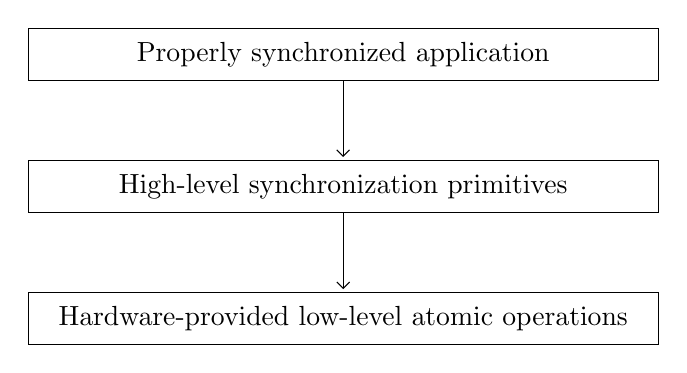
\begin{tikzpicture}[every node/.style={draw, minimum width=8cm, inner sep=0.5em}]
      \node (app) {Properly synchronized application};
      \node [below=of app] (hl) {High-level synchronization primitives};
      \node [below=of hl] (hw) {Hardware-provided low-level atomic operations};
      \draw [->] (app) -- (hl);
      \draw [->] (hl) -- (hw);
    \end{tikzpicture}
  \end{frame}

  \begin{frame}[fragile]
    \frametitle{You Could Use a Lock to Implement Critical Sections}

    Assuming a uniprocessor operating system, you could implement locks as follows:

    \vspace{2em}

    \begin{lstlisting}
void lock() {
  disable_interrupts();
}
void unlock() {
  enable_interrupts();
}   
    \end{lstlisting}

    \vspace{2em}

    This would disable concurrency (assuming it ignores signals and interrupts)

    \hspace{2em} Not going to work on multiprocessors (and OS won't let you change hardware)
  \end{frame}

  \begin{frame}[fragile]
    \frametitle{Let's Try to Implement a Lock in Software}

    \begin{lstlisting}
void init(int *l) {
  *l = 0;
}
void lock(int *l) {
  while (*l == 1);
  *l = 1;
}
void unlock(int *l) {
  *l = 0;
}   
    \end{lstlisting}

    What's the issue with this implementation?

    \vspace{2em}

    \onslide<2->{It's not safe (both threads can be in the critical section)}

    
    \onslide<2->{It's not efficient, it wastes CPU cycles (busy wait)}
  \end{frame}

  \begin{frame}
    \frametitle{You Can Implement Locks in Software with Minimal Hardware}

    You hardware requirements just have to ensure:
    \begin{itemize}
      \item Loads and stores are atomic
      \item Instructions execute in order
    \end{itemize}

    \vspace{2em}

    There's 2 main algorithms you could use:

    \hspace{2em}
    \href{https://en.wikipedia.org/wiki/Peterson\%27s_algorithm}
    {Peterson's algorithm}
    and
    \href{http://en.wikipedia.org/wiki/Lamport\%27s_bakery_algorithm}
         {Lamport's bakery algorithm}

    \vspace{2em}

    The problem is that they don't scale well, and processors execute
    out-of-order
  \end{frame}

  \begin{frame}[fragile]
    \frametitle{Let's Assume a Magical Atomic Function ---
                \texttt{compare\_and\_swap}}

    \texttt{compare\_and\_swap(int *p, int old, int new)} is atomic

    \hspace{2em} It returns the original value pointed to

    \hspace{2em} It only swaps if the original value equals \texttt{old}, and changes it to \texttt{new}

    \vspace{2em}

    Let's give it another shot:

    \begin{lstlisting}
void init(int *l) {
  *l = 0;
}
void lock(int *l) {
  while (compare_and_swap(l, 0, 1));
}
void unlock(int *l) {
  *l = 0;
}   
    \end{lstlisting}
  \end{frame}

  \begin{frame}
    \frametitle{What We Implement is Essentially a Spinlock}

    Compare and swap is a common atomic hardware instruction

    \vspace{2em}

    On x86 this is the \texttt{cmpxchg} instruction (compare and exchange)

    \vspace{2em}

    However it still has this ``busy wait'' problem

    \vspace{2em}

    Consider a uniprocessor system, if you can't get the lock, you should yield

    \hspace{2em} Let the kernel schedule another process, that may free the lock

    \vspace{2em}

    On a multiprocessor machine, it depends
  \end{frame}

  \begin{frame}[fragile]
    \frametitle{Let's Add a Yield}

    \begin{lstlisting}
void lock(int *l) {
  while (compare_and_swap(l, 0, 1)) {
    yield();
  }
  *l = 1;
}
    \end{lstlisting}

    \vspace{2em}

    Now we have a 
    \href{https://en.wikipedia.org/wiki/Thundering_herd_problem}{thundering herd}
    problem

    \hspace{2em} Multiple threads may be waiting on the same lock

    \vspace{2em}

    We have no control over who gets the lock next

    \hspace{2em} We need to be able to reason about it (FIFO is okay)
  \end{frame}

  \begin{frame}[fragile]
    \frametitle{We Can Add a Wait Queue to the Lock}

    \begin{lstlisting}
void lock(int *l) {
  while (compare_and_swap(l, 0, 1)) {
    // add myself to the wait queue
    yield();
  }
  *l = 1;
}
void unlock(int *l) {
  *l = 0;
  if (/* threads in wait queue */) {
    // wake up one thread
  }
}
    \end{lstlisting}

    There are 2 issues with this: 1) lost wakeup, and 2) the wrong thread gets
    the lock
  \end{frame}

  \begin{frame}[fragile]
    \frametitle{Lost Wakeup Example}

    \begin{lstlisting}[numbers=left]
void lock(int *l) {
  while (compare_and_swap(l, 0, 1)) {
    // add myself to the wait queue
    yield();
  }
  *l = 1;
}
void unlock(int *l) {
  *l = 0;
  if (/* threads in wait queue */) {
    // wake up one thread
  }
}
    \end{lstlisting}

    Assume we have thread 1 (T1) and thread 2 (T2), thread 2 holds the lock

    \hspace{2em} T1 runs line 2 and fails, swap to T2 that runs lines 10-12, T1
    runs lines 3 -4

    \hspace{4em} T1 will never get woken up!
  \end{frame}

  \begin{frame}[fragile]
    \frametitle{Wrong Thread Getting the Lock Example}

    \begin{lstlisting}[numbers=left]
void lock(int *l) {
  while (compare_and_swap(l, 0, 1)) {
    // add myself to the wait queue
    yield();
  }
  *l = 1;
}
void unlock(int *l) {
  *l = 0;
  if (/* threads in wait queue */) {
    // wake up one thread
  }
}
    \end{lstlisting}

    Assume we have T1, T2, and T3. T2 holds the lock, T3 is in queue.

    \hspace{2em} T2 runs line 9, swap to T1 which runs line 2 and succeeds

    \hspace{4em} T1 just stole the lock from T3!
  \end{frame}

  \begin{frame}[fragile]
    \frametitle{To Fix These Problems, We Can Use Two Variables (One to Guard)}

    \begin{columns}
      \begin{column}{0.5\textwidth}
        \begin{lstlisting}[basicstyle=\scriptsize\ttfamily]
typedef struct {
  int lock;
  int guard;
  queue_t *q;
} mutex_t;

void lock(mutex_t *m) {
  while (
    compare_and_swap(m->guard, 0, 1)
  );
  if (m->lock == 0) {
    m->lock = 1; // acquire mutex
    m->guard = 0;
  } else {
    enqueue(m->q, self);
    m->guard = 0;
    yield();
    // wakeup transfers the lock here
  }
}
        \end{lstlisting}
      \end{column}
      \begin{column}{0.5\textwidth}
        \begin{lstlisting}[basicstyle=\scriptsize\ttfamily]
void unlock(mutex_t *m) {
  while (
    compare_and_swap(m->guard, 0, 1)
  );
  if (queue_empty(m->q)) {
    // release lock, no one needs it
    m->lock = 0; 
  }
  else {
    // direct transfer mutex
    // to next thread
    wakeup(dequeue(m->q));
  }
  m->guard = 0;
}
        \end{lstlisting}
      \end{column}
    \end{columns}
  \end{frame}

  \begin{frame}
    \frametitle{Remember What Causes a Data Race}

    A data race is when two concurrent actions access the same variable

    and at least one of them is a \textbf{write}

    \vspace{2em}

    We could have any many readers as we want

    \hspace{2em} We don't need a mutex as long as nothing writes at the same
    time

    \vspace{2em}

    We need different lock modes for reading and writing
  \end{frame}

  \begin{frame}
    \frametitle{Read-Write Locks}

    With mutexes/spinlocks, you have to lock the data,

    even for a read since you don't know if a write could happen

    \vspace{2em}

    Reads can happen in parallel, as long as there's no write

    \vspace{2em}

    Multiple threads can hold a read lock ({\tt pthread\_rwlock\_rdlock}),

    but only one thread may hold a write lock ({\tt pthread\_rwlock\_wrlock})

    and will wait until the current readers are done
  \end{frame}

  \begin{frame}[fragile]
    \frametitle{We Can Use A Guard To Keep Track of Readers}

    \begin{columns}
      \begin{column}{0.5\textwidth}
        \begin{lstlisting}
typedef struct {
  int nreader;
  lock_t guard;
  lock_t lock;
} rwlock_t;

void write_lock(rwlock_t *l) (
  lock(&l->lock);
}

void write_unlock(rwlock_t *l) (
  unlock(&l->lock);
}
        \end{lstlisting}
      \end{column}
      \begin{column}{0.5\textwidth}
        \begin{lstlisting}
void read_lock(rwlock_t *l) (
  lock(&l->guard);
  ++nreader;
  if (nreader == 1) { // first reader
    lock(&l->lock);
  }
  unlock(&l->guard);
}
void read_unlock(rwlock_t *l) (
  lock(&l->guard);
  --nreader;
  if (nreader == 0) { // last reader
    unlock(&l->lock);
  }
  unlock(&l->guard);
}
        \end{lstlisting}
      \end{column}
    \end{columns}
  \end{frame}

  \begin{frame}
    \frametitle{We Want Critical Sections to Protect Against Data Races}

    We should know what data races are, and how to prevent them:
    \begin{itemize}
      \item Mutex or spinlocks are the most straightforward locks
      \item We need hardware support to implement locks
      \item We need some kernel support for wake up notifications
      \item If we know we have a lot of readers, we should use a read-write lock
    \end{itemize}
  \end{frame}
\end{document}
